
%(BEGIN_QUESTION)
% Copyright 2007, Tony R. Kuphaldt, released under the Creative Commons Attribution License (v 1.0)
% This means you may do almost anything with this work of mine, so long as you give me proper credit

A valve that is throttling (less than fully open) wastes energy, and so one way to minimize energy usage is to create less upstream pressure so that the control valve operates at a greater opening position.  When the valve in question is a steam valve throttling steam to a load, this means varying the boiler output pressure to keep the throttling valves nearly full open.

$$\includegraphics[width=15.5cm]{i01802x01.eps}$$

Explain how this control system works to maximize energy efficiency, including the role each instrument plays in achieving this goal. 

\underbar{file i01802}
%(END_QUESTION)





%(BEGIN_ANSWER)

This system varies steam header pressure to keep the furthest-open temperature control valve at 90\% opening.  The ZIC should be tuned for slow integral action (little or no proportional action, no derivative action): slower than the PIC, which of course must be slower than the boiler's natural response.  In tuning these controllers, the PIC should be tuned first, then the ZIC.  

It is irrelevant how or when the TIC's are tuned from the perspective of the header pressure control system, as they are not part of the pressure control system, but merely loads.

%(END_ANSWER)





%(BEGIN_NOTES)

This control strategy is similar to that used for controlling variable-speed pumps to keep downstream throttling valves nearly full-open.  It should be noted that the valve position controller (ZIC) needs to have minimal proportional and derivative action, and should control only with slowly-tuned integral action.  The ZIC needs to be significantly slower to respond than the boiler is capable of changing pressure, or else the ZIC will ``chase'' the slow boiler!

\vskip 30pt

Note: this control strategy derived from diagram on page 86 of Francis G. Shinskey's {\it Energy Conservation Through Control}, copyright 1978.

%INDEX% Control, strategies: valve position optimization
%INDEX% Relay, computational: selector functions

%(END_NOTES)


